\documentclass{subfiles}
\begin{document}
\begin{figure}[h!]
    \centering
    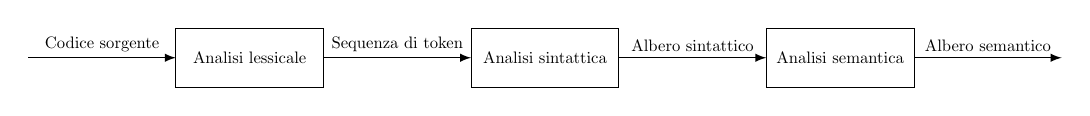
\begin{tikzpicture}[every node/.style={scale=0.6}, scale = 0.75]

        \draw [-latex] (0, 0) -- (2.5, 0);
        \node (n1) at (1.25, 0) [anchor = south] {Codice sorgente};

        \draw (2.5, -0.5) rectangle (5, 0.5);
        \node (n2) at (3.75, 0) [anchor = center] {Analisi lessicale};

        \draw [-latex] (5, 0) -- (7.5, 0);
        \node (n3) at (6.25, 0) [anchor = south] {Sequenza di token};

        \draw (7.5, -0.5) rectangle (10, 0.5);
        \node (n4) at (8.75, 0) [anchor = center] {Analisi sintattica};

        \draw [-latex] (10, 0) -- (12.5, 0);
        \node (n5) at (11.25, 0) [anchor = south] {Albero sintattico};

        \draw (12.5, -0.5) rectangle (15, 0.5);
        \node (n6) at (13.75, 0) [anchor = center] {Analisi semantica};

        \draw [-latex] (15, 0) -- (17.5, 0);
        \node (n7) at (16.25, 0) [anchor = south] {Albero semantico};

    \end{tikzpicture}
    \caption{Struttura di un compilatore.}
    \label{fig:1}
\end{figure}
\end{document}